%=============================================================================
% Thesis Template in LaTex
%
% File:  04-06-Szenarien.tex -- Fallstudie/Modellierung der ungewissen Parameter
% Author(s): Jürgen Hackl <hackl@ibi.baug.ethz.ch>
%            Clemens Kielhauser <kielhauser@ibi.baug.ethz.ch>
%
% Creation:  27 Jan 2014
% Time-stamp: <Tue 2013-08-13 20:14 juergen>
%
% Copyright (c) 2014 Infrastructure Management Group (IMG)
%               http://ibi.ethz.ch
%
% More information on LaTeX: http://www.latex-project.org/
%=============================================================================

% Unterkapitel Szenarien
% ---------

\subsubsection*{Bevölkerungswachstum}
\label{subsubsec:Bevölkerung}

Wie unter Abschnitt \ref{chap:Fallstudie} erwähnt, ist das DTV abhängig von der zukünftigen demographischen Entwicklung.
Um den Effekt den das Bevölkerungswachstum auf das DTV haben wird, modellieren zu können orientiere ich mich an den Wachstumsprognossen.
Die zu erwartende Bevölkerungsentwicklung habe ich dem Kapitel 3 \textit{Stadt Uster im Porträt} des STEK Schlussbericht entnommen und wird nachfolgend kurz beschrieben. Anhand dieser Beschreibung und unter der Annahme eines linearen Wachstums berechne ich das DTV für den MIV und den Langsamverkehr, sprich die Velofahrer.


\begin{description}
\item[Stagnation] \hfill \\
Geschätzte Anzahl an Einwohner im Jahr 2035 beträgt 38'760, somit wächst die Bevölkerung jährlich um 188 Einwohner bzw. um 0.5\% gegenüber 2015
\item[Trend restriktiv] \hfill \\
Geschätzte Anzahl an Einwohner im Jahr 2035 beträgt 42'260, somit wächst die Bevölkerung jährlich um 363 Einwohner bzw. um 1\% gegenüber 2015
\item[Trend Prosperität] \hfill \\
Geschätzte Anzahl an Einwohner im Jahr 2035 beträgt 45'620, somit wächst die Bevölkerung jährlich um 531 Einwohner bzw. um 1.5\% gegenüber 2015
\end{description}

Anhand dieser Wachstumsprognossen, bilde ich die drei nachfolgend dargestellten Szenarien. Mit diesen Szenarien werde ich in einem nächsten Schritt den zukünftigen DTV am Bahnübergang Brunnenstrasse ermitteln.

\begin{itemize}
\item Szenario: SB 1
	\begin{itemize}
	\item Grundlage: Stagnation $\Rightarrow$ jährliches Wachstum um 0.5\%
	\item Eintrittswarscheinlichkeit: 25\%
	\end{itemize}
\item Szenario: SB 2
	\begin{itemize}
	\item Grundlage: Trend restriktiv  $\Rightarrow$ jährliches Wachstum um 1 \%
	\item Eintrittswarscheinlichkeit: 50\%
	\end{itemize}
\item Szenario: SB 3
	\begin{itemize}
	\item Grundlage: Trend Prosperität  $\Rightarrow$ jährliches Wachstum um 1.5\%
	\item Eintrittswarscheinlichkeit: 25\%
	\end{itemize}
\end{itemize}

Die Wahrscheinlichkeit das Szenario SB 2 eintritt und der DTV jährlich um 120 Fahrzeuge zunimmt, bewerte ich mit 50\%. Dies geschieht unter der Annahme, dass der restriktive Trend das minimale Wachstumsziel von 20\% wiederspiegelt, welches gemäss dem STEK mit grösster Wahrscheinlichkeit eintretten wird und das dieses Szenario dem kantonalen Prognossen entspricht. 
Das es zu einem verstärktem Wachstum von 1.5\% und somit zu einer Zunahme von 180 Fahrzeugen am DTV pro Jahr kommt, erachte ich nach den Angaben des STEK als unwahrscheinlich, da ein übermässiges Bevölkerungswachstum, aufgrund der nur beschränkt vorhandenen Kapazitäten zur Erweiterung der Wohnangebots, nur bedingt möglich ist. Das es zu einer Stagnation des Bevölkerungswachstums und im Zuge dieser Modellierung zu einem Verkehrswachstum von 0.5\% und einer Zunahme von 60 Fahrzeugen am DTV pro Jahr, kommt, erachte ich in Anbetracht der Prognossen zur demographische Entwicklung im Kanton Zürich, als unwahrscheinich. Deshalb bewerte ich die Szenarien SB 1 und SB 3 mit jeweils 25\%.

Mithilfe der verschiedenen Wachstumsraten $WR_{s}$ der Szenarien und der Formel \ref{eq.11} berechne ich das $DTV_{i}$ im Jahr $t_{i}$.

\begin{equation*}
DTV_{i} = DTV_{2016} + \bigl( t_{i} - t_{2016} \bigr) \cdot \bigl[WR_{s}\bigr] \cdot DTV_{2016}
\label{eq.11}
\end{equation*}

Gemäss GIS-Browser lag der durchschnittliche Werkverkehr im Jahr 2016 bei 12'023 Fahrzeugen. Diesen Wert benutzte ich als Startwert sowie Basiswert meiner Berechnungen. Da die Anzahl Velos, die den Bahnübergang an der Brunnenstrasse täglich passieren, nicht von einer Verkehrsmessstelle gezählt wird, muss diese Information aus der Menge an Autos hergeleitet werden. Dies erfolgt mithilfe der Daten der Verkehrsmessstelle an der etwas südlich von Uster gelegenen Seefeldstrasse, welche Niederuster mit Riedikon verbindet. 
Der im Jahr 2019 gemessen durchschnittliche DTV lag bei 8818 Motorfahrzeugen und 913 Velofahrer. Daraus ergibt sich einen Veloanteil von 10.35\%. \footcite{MIVSeefeld}\footcite{VeloSeefeld}

\begin{align*}
\mu &= \frac{DTV_{Velo,Seefeldstrasse}}{DTV_{MIV,Seefeldstrasse}}   \\
DTV_{Velo} &= DTV_{MIV} \cdot \mu_{Velo} 
\end{align*}

In den Abbildung \ref{fig:DTV} sind die Ergebnisse meiner Modellierung des DTV am Bahnübergang Brunnenstrasse dargestellt. Mit diesen Werten habe ich die Berechnung der Kosten und schlussendlich die Optimierung der Zielfunktion vorgenommen.

\begin{figure}[h!]
  \centering
  \subfloat[][]{\label{fig:04-06-02-DTV(MIV)}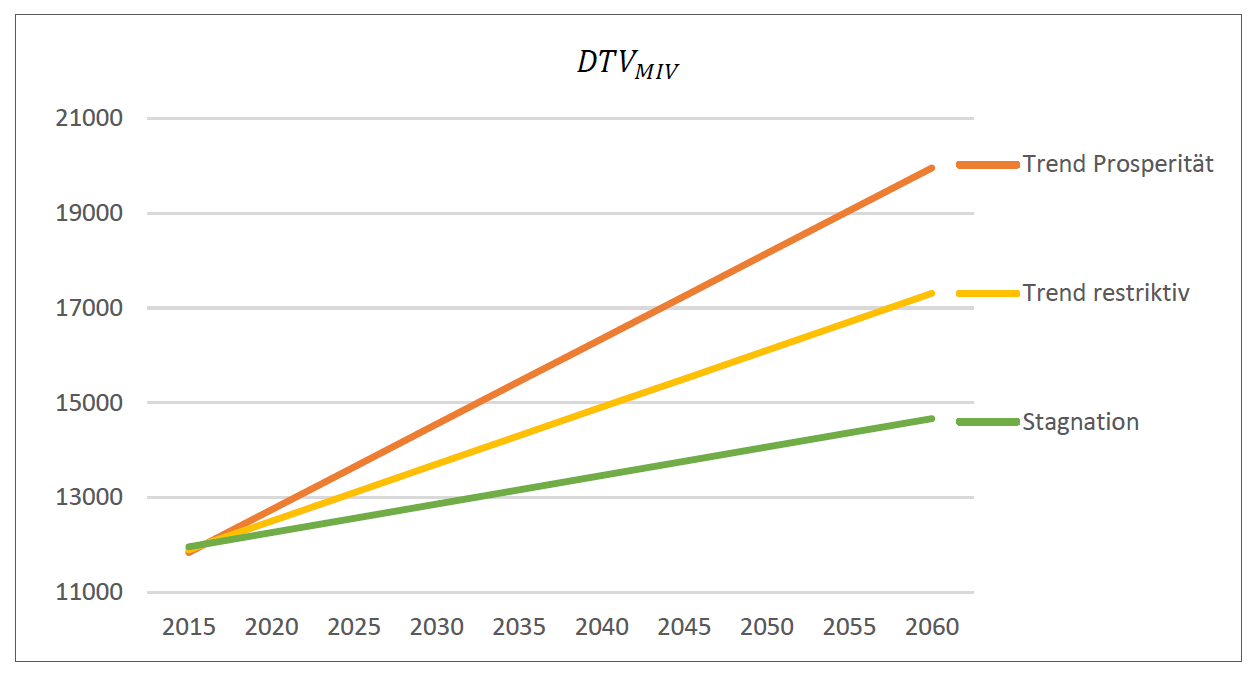
\includegraphics[width=.45\textwidth]{./figures/04-06-02-DTV(MIV)-SzenarienBev.Wachstum}}
  \hfill
  \subfloat[][]{\label{fig:04-06-03-DTV(VELO)}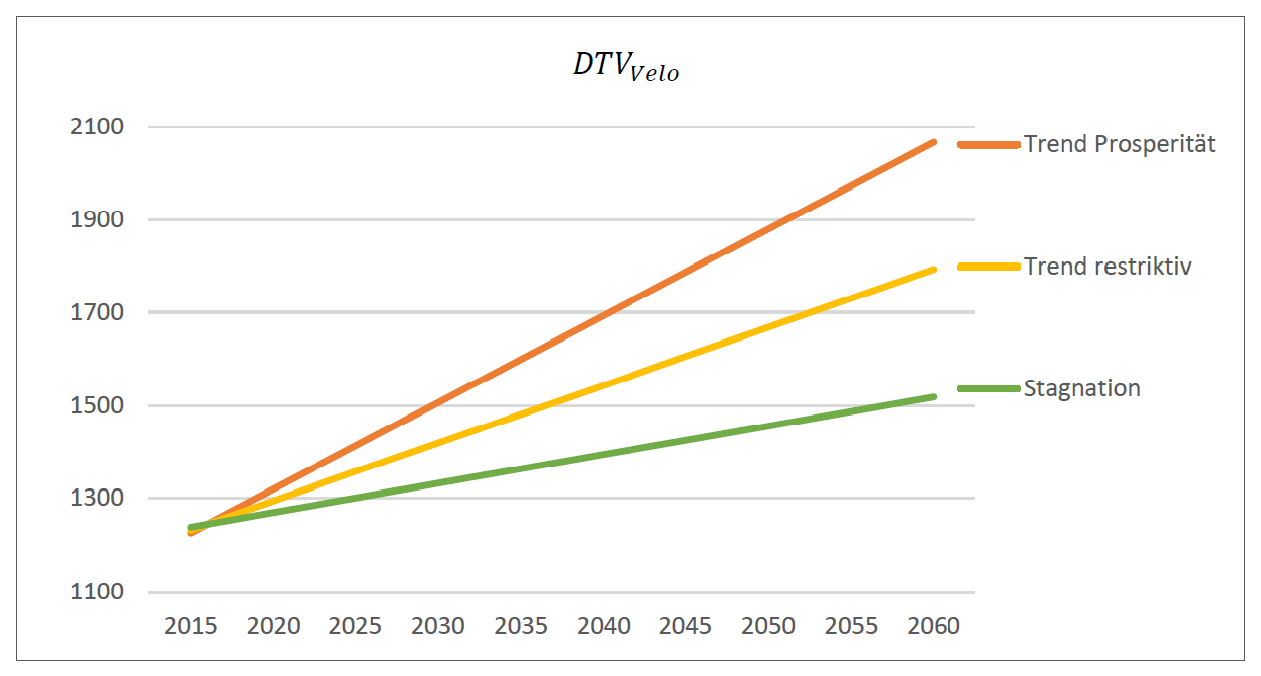
\includegraphics[width=.45\textwidth]{./figures/04-06-03-DTV(VELO)-SzenarienBev.wachstum}}
\caption[Verkehrsaufkommen]{Tägliches Verkehraufkommen Brunnenstrasse}
  \label{fig:DTV}
\end{figure}

\newpage


\subsubsection*{Umsetzung der STEK}
\label{subsubsec:Umsetzung}


Den Effekt der die Umsetzung der Leitziele der STEK auf den täglichen Velo-Mehrverkehr haben wird, modelliere ich anhand der folgenden Szenarien. Das meines erachtens mit der grössten Wahrscheinlichkeit eintrettende Szenario, entspricht der Verkehrsprognosse des Bundes, die eine Zunahme des Langsamverkehrs von 2015 bis 2040 um 32\% erwartet. (\cite{Perspektive2040}) 
Um die Ober- sowie Untergrenze meiner Prognosse ermitteln zu können, orientiere ich mich ein weiteres mal an dem STEK. Mithilfe der unter Kapitel 10 \textit{Stadt Uster im Porträt} des STEK vorgestellten Wachstumsprognossen für die Bevölkerungsentwicklung sowie der in Kapitel 7 \textit{Mobilität} der STEK gemäss regionalem Richtplan erstellten Verkehrsprognosse für den Anteil der Velofahrer am Gesamtverkehr, erstelle ich zwei weitere Szenarien. 
Einerseits berücksichtige ich den Fall einer ungenüngenden Umsetzung der Leitziele und der daraus resultierenden stagnierenden Entwicklung des Veloverkehr. Andererseits den Fall einer maximalen Umsetzung aller Ziele in Verbindung mit einer Verschiebung des Innerstädtischen Modal-Split in Richtung Langsamverkehr.

\begin{description}
\item[Stagnation] \hfill \\
Prognosse gemäss STEK: $\rightarrow$ jährliches Wachstum: 0.54 \% 
\item[Verkehrsperspektiven 2040] \hfill \\
Prognostiziertes Wachstum bis 2040: 32\% $\rightarrow$ jährliches Wachstum: 1.3 
\item[Umsetzung maximal] \hfill \\
Prognosse gemäss STEK und regionalem Richtplan: $\rightarrow$ jährliches Wachstum: 2 \% 
\end{description}

Das Eintretten einer Stagnation erachte ich, unter berücksichtigung der Entwicklung des Langsamverkehr über die letzten zehn Jahre, als unwahrscheinlich und bewerte diese Prognosse daher mit 5\%.
Das es zu einem Wachstum gemäss der Prognosse des Bundes kommen wird, erachte ich nach der Konsultation weitere Verkehrsprognossen, als das Szenario, welches mit grössten Sicherheit eintretten wird. Daher bewerte ich diese Szenario mit einer Eintrittswahrscheinlichkeit von 57.5\%. 
Das alle Ziele maximal erfüllt werden und eine Verschiebung des Innerstädtischen Modal-Split statt findet, erachte ich mit 32.5\% als deutlich plausibler als die Stagnation, jedoch als unwahrscheinlichr als die Prognosse des Bundes. 

\begin{itemize}
\item Szenario: SU 1
	\begin{itemize}
	\item Grundlage: Stagnation 
	\item Eintrittswarscheinlichkeit: 5\%
	\end{itemize}
\item Szenario: SB 2
	\begin{itemize}
	\item Grundlage: Verkehrsperspektiven 2040
	\item Eintrittswarscheinlichkeit: 57.5\%
	\end{itemize}
\item Szenario: SB 3
	\begin{itemize}
	\item Grundlage: Umsetzung maximal
	\item Eintrittswarscheinlichkeit: 32.5\%
	\end{itemize}
\end{itemize}

Anhand der zu Beginn dieses Abschnitts definierten Wachstumsraten, ausgehend von den Messwerte des täglichen Veloverkehr im Jahr 2016, habe ich die Anzahl Velos, die in jedem Szenario zusätzlich pro Tag auf der Infrastruktur unterwegs sein werden, ermittelt. Die Anzahl Velos die im Jahr 2016 täglich den Bahnübergang nutzten, lag, gemäss Abschnitt \ref{subsubsec:Demographie}, bei 1245.
Somit führt das Szenario SU 1 zu einer Erhöhung des täglichen Veloverkehr um 7 Velos, das Szenario SU 2 zu einer Zunahme von 16 Velos und das Szenario SB 3 zu einer Erhöhung des tägliche Veloverkehrs um 25 Velos. 
Mit diesen Angaben berechne ich die Anzahl Velos, die je nach Szenario, zusätzlich zu den in Abschnitt \ref{subsubsec:Demographie} berechneten DTV-Werten, auf der Infrastruktur verkehren werden.


% ===========================================================================
% EOF
%

%%% Local Variables:
%%% mode: latex
%%% TeX-master: "../main"
%%% End:
